\newpage
\changeindent{0cm}
\section{コミック工学に関連するデータセット}
\changeindent{2cm}

本章では, コミック工学に関連するデータセットについて説明する.

\changeindent{0cm}
\subsection{Manga109}
\changeindent{2cm}

Manga109 \cite{mtap_matsui_2017} は,
漫画の研究のために相澤らにより作られたもので, 日本のプロの漫画家によって描かれた 109 冊の漫画で構成されており, これらは 1970 年代から 2010 年代に公開された漫画であり, 対象読者層やジャンルも幅広く網羅している. Manga109 には 109 冊の漫画の画像データや登場人物の名前, 画像内における登場人物の顔, 全身, コマ, テキストの座標などのアノテーションデータが含まれている.
しかし, Manga109 には
セリフの発話者に関する情報や, 本研究の趣旨であるセリフの感情に関する情報は付与されていない.

\changeindent{0cm}
\subsection{4 コマ漫画ストーリーデータセット}
\changeindent{2cm}

4 コマ漫画ストーリーデータセット \cite{ueno_miki2018} は, 上野によって作られた, コミック工学発展のために研究者が
一から開発に関わった世界初の研究用のデータセットであり, 画像データのレイヤー分けや作者によるセリフの感情アノテーションなど, いくつかの特徴がある.

Manga109 といった市販コミックによって構成
されたデータセットとは異なり, 4 コマ漫画ストーリーデー
タセットのデータは本データセットのために幾人かの
漫画家によって描き下ろされている. 市販されたコミッ
クをデータとした場合, 著作権などの問題に加え, 計
算機上で扱うためのデータが少なく, コミックの意味
理解を目的とした研究には適さないという問題がある.
例えばコミックに登場するキャラクターの感情は明示
されていないため, 読者によるアノテートによってラベ
ルを付与する必要があるが, アノテートされたラベル
が漫画家の意図とは異なる可能性を否定できない. ま
た, マルチモーダルでストーリーの解析をする際にオ
リジナリティの観点から同一プロットを複数の漫画家
が描くことは稀有なため, そういったデータの収集に
基づく研究は困難である. 4 コマ漫画ストーリーデータセットは
そういった問題点を解決するために作られたデー
タセットである.

上野は4 コマ漫画の構造を,

\begin{itemize}
  \item 一般:標準的な起承転結をもつ
  \item 繰り返し:1, 2 コマ間の類似が 3, 4 コマ間でも起きる
  \item 出オチ:1 コマ目におかしな絵が描かれてオチがある
  \item タイトルオチ:最後にタイトルを見返してオチがわかる
  \item 再帰:4 コマ目から1 コマ目に戻り話として成立する
  \item 参照:1 つ以上前の話の続きの話となる
  \item 連続した 4 コマを 2 話並べて 8 コマで話となる
\end{itemize}

と定義し, これに従ってデータセットを作成している.
現在は, 同一のストーリーを 4 コマ目がオチとなる一
般と出オチの 2 つの構造から描いたものがデータとし
て存在している.

また, 上野は異なる作者によって描かれた4 コマ
漫画を, そのタッチを基に

\begin{itemize}
  \item ギャグタッチ
  \item 少女漫画タッチ
  \item 少年漫画タッチ
  \item 青年漫画タッチ
  \item 萌えタッチ
\end{itemize}

と分類した. また, 各タッチにつき 10 話ずつ存在する. 図 \ref{fig:4koma_data} に,
4 コマ漫画ストーリーデータセットのデータ例を示す.

\newpage
\begin{figure}[!h]
  \centering
  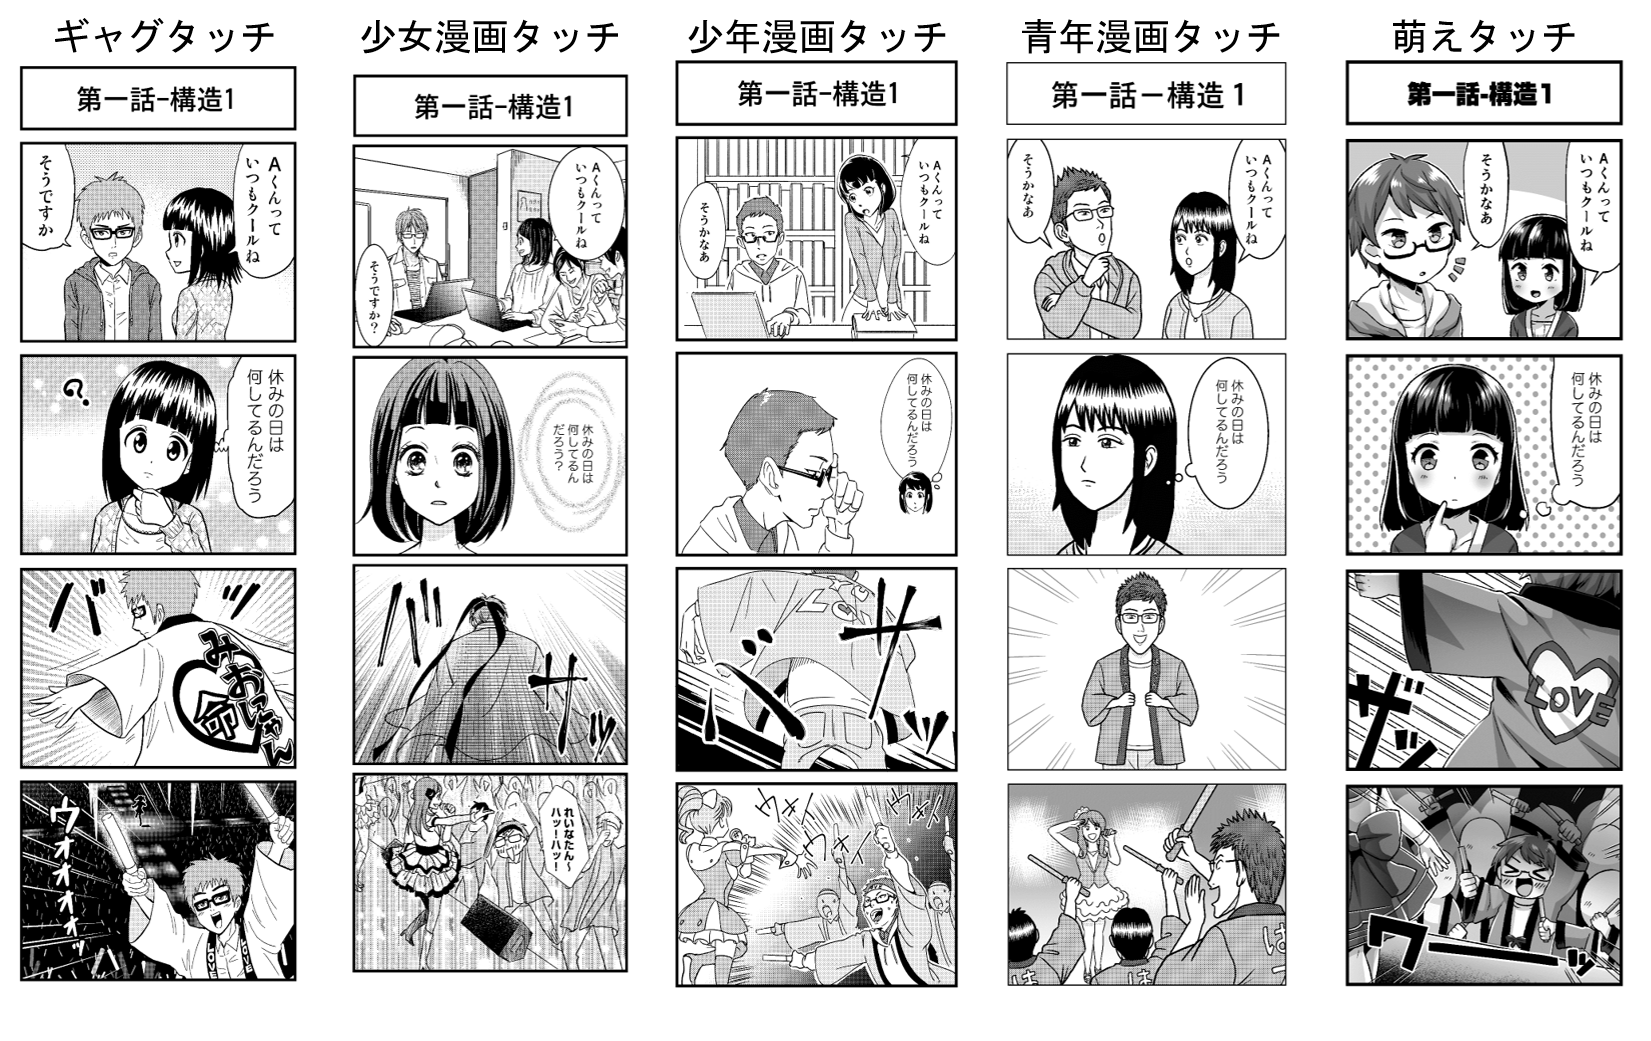
\includegraphics[width=0.8\hsize]{doc/figures/4koma_data.png}
  \caption{4 コマ漫画ストーリーデータセットのデータ例}
  \label{fig:4koma_data}
\end{figure}

\begin{flushleft}
\begin{center}
ギャグタッチ : \copyright 作画:浦田カズヒロ \\
少女漫画タッチ : \copyright 作画:高科りさ \\
少年漫画タッチ : \copyright 作画:鈴木市規 \\
青年漫画タッチ : \copyright 作画:湯沢としひこ \\
萌えタッチ : \copyright 作画:棟田ウメコ \\
シナリオ:(株) スポマ播村早紀 / 大阪工業大学 上野未貴 \\
\end{center}
\end{flushleft}
